\chapter{Introduction}
While approaching a more and more ubiquitous network experience where we are
connected to different personal area networks (PAN) or even the global internet
around the clock two problems become more important. One problem is the power
consumption of devices which make the ubiquity possible. In contrast to other
computing devices we want them to be well hidden and unintrusive. Changing
batteries or having power cables around is not a real option for them. On the
other hand wireless communication protocols with IEEE 802.11 \cite{ieee80211} as the
leading option are a good choice for mobile devices like notebooks or
smartphones but are still to power hungry for small ubiquitous devices.
With IEEE 802.15.4 \cite{ieee802154} a new protocol was designed for exactly such
small, power constraint devices. We will use it in our research and have some
more information about it prepared in section~\ref{intro802154}.

The second problem are network connection disruptions - be it due to movement or
the other changes. The most widely used protocol family with IP, UDP, TCP is not
designed to cope with disrupted networks. They need an established physical connection
to work as expected. If this is not the case the packets may be just lost
as in case of UDP or have to be re-transmitted. This re-transmission could be
problematic if the network connection is unavailable more often then available.
For such scenarios delay tolerant networking was designed to send the
packets, perhaps over several hops, to the destination without needing to
establish a channel between source and destination. In~\ref{introdtn} we give a
short introduction to DTN before describing the IBR-DTN implementation in chapter
\ref{ibr-dtn} and our convergence layer in chapter \ref{802154layer}.

\section{IEEE 802.15.4}
\label{intro802154}
Driven by an IEEE working group the IEEE 802.15.4 standard provides the physical and
media access control layer for so called low-rate wireless personal area network
(LR-WPAN). The emphasis is on low cost devices for communication without
infrastructure over small distances. The offered transfer rate can be up to 250 kbps.
The standard specifies three possible frequency bands to operate in. 16 channels
in the 2450 MZz band, 10 channels in the 915 MHz band and one channel in the 868
MHz band. The usage of some may be restricted in different countries but 2450 MHz
band is available worldwide.
Other features of IEEE 802.15.4 includes collision avoidance through CSMA/CA, built
in support for secure communication through cryptography, power management through
link quality control and energy detection as well as acknowledgements,
retransmissions and reserved time slots for real-time operations.

As already described the standard only covers the two lowest layer of a
protocol stack. Supplementing it to a fully functional networking stack is the aim
of different other specifications as shown in figure~\ref{fig:802154layer}. The
most widely know is be ZigBee. With 6LowPAN there is also work underway to combine
LR-WPAN with standard internet protocols like IPv6.

Specified for an infrastructure-less network the topologies may be star or
Peer-to-Peer based as well a combination of both. Figure \ref{fig:802154topologies}
shows examples for these topologies. Two different device types are allowed:
full-function device (FFD) and
reduced-function device (RFD). The RFD is a very simple device which can only
connect to one FFD at a time. Therefore it can only act as a leaf in all
described topologies. In contrast, the FFD is able to act as a coordinator to
create a new PAN and relay messages to other nodes. At least one coordinator
is needed in every network. It creates the network and assigns addresses to
associating nodes. These assigned addresses are short addresses with only 16 bit
and only unique withing the PAN. Additionally every node has a long address with
64 bit unique worldwide. One thing to keep in mind is that routing is not
covered by the standard. To relay messages over multiple hops the supplementing
upper layers need to take care of this.

\begin{figure}
  \begin{center}
    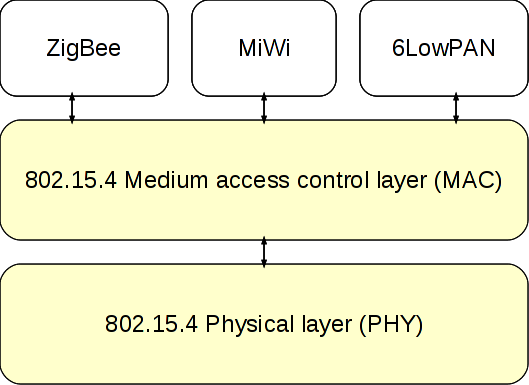
\includegraphics[height=6cm]{images/802154layer}
    \caption{IEEE 802.15.4 lower layers with optional upper layers}
        \label{fig:802154layer}
  \end{center}
\end{figure}

\begin{figure}
  \begin{center}
    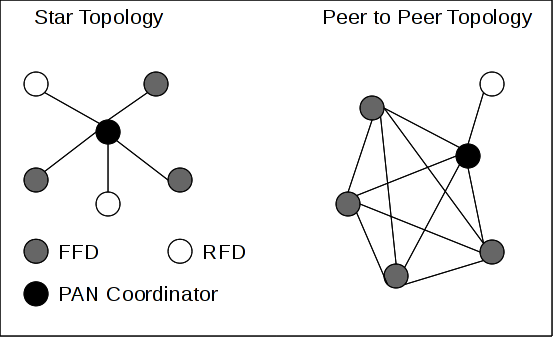
\includegraphics[height=6cm]{images/802154topology}
    \caption{IEEE 802.15.4 network topologies}
        \label{fig:802154topologies}
  \end{center}
\end{figure}

\section{DTN}
\label{introdtn}
The need for communication between nodes without continuous network
connectivity is what DTN seeks to address. Most modern routing protocols only
send out the payload once a complete route to the destination has been established.
A communication over such an approach is only possible if source and destination
are connected to a network long enough to establish a route between them,
transfer the data and possibly acknowledge the transfer.

DTN in contrast uses a store and forward approach which sends out the data
together with the destination address. The bundle protocol in
\cite{RFC5050} was specified for this. One approach to maximize the probability
of a successful delivered message would be to send out multiple copies of the
same message, maybe to different hops. Such an approach obviously increases the
network and storage load and may not be useful for constrained devices like
sensor nodes.

The bundle protocol specifies an overlay network which interacts with the lower
layers over convergence layers. The lower layers are not bound to be IP
based even if that is the one widely used. In this thesis we describe the usage
of the DTN implementation IBR-DTN over an IEEE 802.15.4 radio link on a Linux
based system.

\section{Related Work}
\label{relatedwork}

While DTN is becoming more popular for research there are only a few research
projects which combine DTN with sensor network technologies like IEEE 802.15.4.
This is not surprising if one keeps in mind that the DTN architecture is
complex and memory as well as bandwidth consuming. Both resources that are scare
on sensor network platforms.

Two projects are aiming to explore this area of research. One of them is the
TinyOS based DTNLite \cite{dtnlite}. It is loosely based on the DTN overlay
architecture. To deliver custody transfer over the overlay they use techniques
like asynchronous message delivery. The concept is targeted at data collection
applications which need to reach a central station for the collection over the
network. The applications must be written or re-written to be DTNLite aware.

ContikiDTN \cite{contikidtn} is, like DTNLite, written for a special purpose
embedded operating system (in this case Contiki
\footnote{http://www.sics.se/contiki/}). While DTNLite only aims to work with
other DTNLite installations, ContikiDTN aims for full standard compliance.
ContikiDTN is tied to only work with a TCP convergence layer. It was a design
choice that no other convergence layer can be plugged in. This restriction is based in
the usage of Contiki's µIP component which offers only TCP protosockets

Both implementations have not been suitable for our work as they are either not
standard compliant or have a design restriction to only use TCP. Furthermore both
are designed around a special purpose operating system while our aim was to work
on the general purpose operating system Linux.
